%%%%%%%%%%%%%%%%%%%%%%%%%%%%%%%%%%%%%%%%%%%%%%%%%%%%%%%%%%%%%%%%%%%%%%

% Paper 2

% POLARIZATION

%%%%%%%%%%%%%%%%%%%%%%%%%%%%%%%%%%%%%%%%%%%%%%%%%%%%%%%%%%%%%%%%%%%%%%

\documentclass[useAMS,usenatbib,a4paper,onecolumn]{mn2e}

\voffset=-0.6in

% Packages:
\input psfig.sty
\usepackage{xspace}
\usepackage{graphicx}
\usepackage{amssymb}
\usepackage{amsmath}

% Macros:
% Making life easier
\newcommand{\be}{\begin{equation}}
\newcommand{\ee}{\end{equation}}
\newcommand{\bs}{\begin{split}}
\newcommand{\bea}{\begin{eqnarray}}
\newcommand{\eea}{\end{eqnarray}}

% Useful symbols
\newcommand{\om}{\Omega_m}
\newcommand{\ha}{\frac{1}{2}}
\newcommand{\ahub}{\frac{\dot{a}}{a}}
\newcommand{\ode}{\Omega_{de}}
\newcommand{\Oe}{\Omega_{e}}
\newcommand{\lcdm}{$\Lambda$CDM}
\newcommand{\neff}{N_{\rm eff}}
\newcommand{\hfid}{H^2_{\rm fid}}
\newcommand{\dl}{\delta}
\newcommand{\sumu}{\Sigma m_\nu}
\newcommand{\mnu}{\Sigma m_\nu}
\newcommand{\mpci}{\,{\rm Mpc}^{-1}}

\newcommand{\dataext}{\data_{\rm ext}}
\newcommand{\transferext}{\mathbf{R}_{\rm ext}}
\newcommand{\smat}{\mathbf{S}}
\newcommand{\cmat}{\mathbf{C}^{\epsilon}}
\newcommand{\cmatext}{\mathbf{C}^{\epsilon_{\rm ext}}}
\newcommand{\noisemat}{\mathbf{N}^{\epsilon}}
\newcommand{\noisematext}{\mathbf{N}^{\epsilon_{\rm ext}}}
\newcommand{\noisematinv}{\left(\noisemat\right)^{-1}}
\newcommand{\noisemattransfer}{\tilde{\mathbf{N}}^{\epsilon}}
\newcommand{\noisemattransferext}{\tilde{\mathbf{N}}^{\epsilon_{\rm ext}}}
\newcommand{\noisemattransferinv}{\left(\tilde{\mathbf{N}}^{\epsilon}\right)^{-1}}
\newcommand{\noisemattransferextinv}{\left(\tilde{\mathbf{N}}^{\epsilon_{\rm ext}}\right)^{-1}}

% Macros
\newcommand{\half}{\frac{1}{2}}
\newcommand{\rhocrit}{\rho_{\rm crit}}
\newcommand{\rvir}{r_{\rm vir}}
\newcommand{\mvir}{m_{\rm vir}}
\newcommand{\kv}{\mathbf{k}}
\newcommand{\xv}{\mathbf{x}}
\newcommand{\mv}{\mathbf{m}}
\newcommand{\muv}{\bm \mu}
\newcommand{\hmsun}{h^{-1}M_{\odot}}
\newcommand{\hmpc}{h^{-1}Mpc}
\newcommand{\hgpc}{h^{-1}{\rm Gpc}}

%%% "Data" - i.e., the observed CMB temperature map
\newcommand{\data}{\mathbf{d}}
%%% Parameters: gravitational potential
\newcommand{\Pot}{\Phi}
\newcommand{\Potvector}{\boldsymbol{\Pot}}
%%% "Signal" - i.e., zero-noise CMB temperature
\newcommand{\signal}{\mathbf{s}}
%%% "noise" - i.e., the pixel noise realization
\newcommand{\noise}{\mathbf{n}}
%%% Transfer function relating the 3D gravitational potential to the
%%% 2D CMB temperature (or other) map
\newcommand{\transfer}{\mathsf{R}}
%%% Signal and noise covariance matrices
\newcommand{\Smat}{\mathsf{S}}
\newcommand{\Nmat}{\mathsf{N}}
\newcommand{\Psimat}{\mathsf{\Psi}}
\newcommand{\Sigmamat}{\mathsf{\Sigma}}
\newcommand{\Cmat}{\mathsf{C}}
%%% Gravitational potential represented as a vector of "voxels" or similar
\newcommand{\gravpot}{\bm \Psi}
%%% Normal (Gaussian) distribution
\newcommand{\normdist}{\mathcal{N}}
%%% Probability theory
\newcommand{\pr}{{\rm Pr}}


%%%%%%%%%%%%%%%%%%%%%%%%%%%%%%%%%%%%%%%%%%%%%%%%%%%%%%%%%%%%%%%%%%%%%%

\title[Inflation from the 3D Potential of the Universe]
{The Music of the Sphere: Connecting the Potential of the Universe on the Largest Scales to Inflation}

\author[Levasseur et al.]{%
    Laurence Perrault Levasseur$^{1}$\thanks{\lplemail}
    Roger~D.~Blandford,$^{1}$
    Philip~J.~Marshall,$^{1}$
    \medskip\\
    $^1$\kipac
}

%%%%%%%%%%%%%%%%%%%%%%%%%%%%%%%%%%%%%%%%%%%%%%%%%%%%%%%%%%%%%%%%%%%%%%

\begin{document}

\date{to be submitted to arxiv}
\pagerange{\pageref{firstpage}--\pageref{lastpage}}\pubyear{2015}

\maketitle

\label{firstpage}

%%%%%%%%%%%%%%%%%%%%%%%%%%%%%%%%%%%%%%%%%%%%%%%%%%%%%%%%%%%%%%%%%%%%%%

\begin{abstract}

Abstract goes here.

\end{abstract}

% Full list of options at http://www.journals.uchicago.edu/ApJ/instruct.key.html

\begin{keywords}
  cosmology
\end{keywords}

\setcounter{footnote}{1}


%%%%%%%%%%%%%%%%%%%%%%%%%%%%%%%%%%%%%%%%%%%%%%%%%%%%%%%%%%%%%%%%%%%%%%

\section{Definitions and Constants}

Inflation provides a way of seeding perturbations to the metric outside the Hubble horizon (well) before the time of BBN. It is common to quantify these perturbations with the gauge-invariant curvature perturbation of the metric $\zeta$, which is defined by:
\be
	-\zeta=\psi+H\frac{\delta\rho}{\rho}\, ,
\ee
where $\psi$ is the trace part of the spatial scalar metric perturbations, i.e. writing the most general spatial perturbation to a 4-d metric by $\delta g_{ij}=2(\psi\delta_{ij}-E_{ij})$ with $\nabla^2E=0$, then $\psi$ contains the trace of the perturbation. We also define $\rho$ and $\delta \rho$ to be the mean energy density and the linear energy density perturbation, respectively, as well as the $H$, the Hubble parameter. $H$ and $\rho$ are related through the first Friedmann equation,
\be
\label{eq:Hubbledef}
	H^2\equiv \left(\frac{\dot{a}}{a}\right)^2=\frac{1}{3\Mp}\rho=\frac{1}{3\Mp}\left( \frac{\dot\varphi^2}{2}+\frac{1}{2}\frac{\nabla^2\varphi}{a^2}+V \right)\, ,
\ee
 where a is the scale factor and, in the third equality, we have related $\rho$ to the field content of the Universe assuming a single scalar field, $\varphi$, is dominating its energy density, as is the case in single field inflation. The 3 terms in the l.h.s. of (\ref{eq:Hubbledef}) represent, in order of appearance, the kinetic energy density of the field, its gradient energy density, and its potential energy.

 For inflation to occur, the field $\varphi$ must be dominated by its homogeneous mode, hence at the background level one has $\frac{1}{2}\frac{\nabla^2\varphi}{a^2}=0$, and its potential energy must dominate over its kinetic energy density. Hence $\dot\varphi^2\ll V$ during inflation. Moreover, during single-field inflation, there is only one physical scalar perturbation degree of freedom representing both scalar metric fluctuations and $\varphi$ fluctuations. Therefore, through an appropriate gauge choice, it is possible to gauge away all linear fluctuations in $\varphi$ and be left with only $\zeta$ as the scalar perturbation. This gauge choice is commonly called the $\zeta$-gauge, or comoving gauge.

During inflation, $H$ remains almost constant, since $V\gg\dot\varphi^2$ and $\varphi$ is almost static. Deviations from $H=\,$cst can be quantified by a hierarchy of slow-roll parameters:
\be
	\epsilon\equiv-\frac{\dot H}{H^2}\, ;\quad \eta=\frac{\dot \epsilon}{\epsilon H}\, ; \quad \eta_n=\frac{\dot{\eta}_{n-1}}{\eta_{n-1}N} ~~\mathrm{for~}n>1\, .
\ee
Inflation requires $\epsilon<1$, and obtaining at least 60 $e$-folds requires $\eta<1$ as well. In the case of single-field inflation, which we will assume in the rest of these notes, the first slow-roll parameter $\epsilon$ can also be re-written as:
\be
	\epsilon=\frac{1}{2}\frac{\dot\varphi^2}{\Mp^2H^2}\, ,
\ee
a formula that will be very useful in the following. Moreover, it will prove useful to use this to re-write $H$ as a function of $\epsilon$ and $V$ only:
\be
\label{eq:HnVrel}
	\Mp^2H^2=\frac{V}{3-\epsilon}
\ee

\bigskip
The main observable predicted by inflation is the power spectrum of curvature fluctuations, $\mathcal{P}_\zeta (k)$, defined by:
\be
	\langle \zeta_k \zeta_k'\ \rangle=(2\pi)^{(3)}\delta^3(k+k')\mathcal{P}_\zeta(k)
\ee
Explicitly, $\mathcal{P}_\zeta (k)$ can be calculated to be
\be
	\mathcal{P}_\zeta(k)=\left.\frac{1}{4 k^3}\frac{H^2}{\epsilon}\right|_{k=aH}\, .
\ee
Quantities in the above equation are evaluated at horizon exit for every mode. Since each mode $\zeta_k$ remains constant outside of the Hubble horizon (see, e.g. Weinberg's proof in astro-ph/0302326), it is sufficient to calculate the amplitude of each mode at horizon exit and fix it from there until horizon re-entry, much after inflation.  If we do not want to perform the evaluation at horizon crossing, it is also possible to write an expression involving the explicit $k$-dependence, through a Hankel function of the first kind:
\be
	\mathcal{P}_\zeta(k)\sim \frac{\pi}{2}(-\tau)^{2\nu}\left| H^{(1)}_\nu(-k\tau)\right|^2\, .
\ee
Here, $\tau$ is the conformal time, related to the cosmic time $t$ by $dt=ad\tau$, and $\nu$ is given by:
\be
	\nu=\frac{3}{2}+\epsilon+\frac{1}{2}\eta
\ee
to leading order in slow-roll parameters.
The dimensionless form of the power spectrum is given by
\be
	\Delta^2_\xi\equiv\frac{k^3}{2\pi^2}\mathcal{P}_\zeta(k)\,.
\ee


Other useful observables to define are the tilt of the power spectrum, defined by:
\be
	n_s-1\equiv\frac{d\ln\Delta^2_\zeta}{d\ln k}=-\epsilon-2\eta\, ,
\ee
where the last equality holds to first order in slow-roll parameters, and the running, defined by (to leading order in slow roll)
\be
	\alpha_s=-2\eta\epsilon-\eta\eta_2\, .
\ee
Finally, the tensor-to-scalar ratio is given by:
\be
	r=16\epsilon\, .
\ee
The amplitude of the power spectrum is usually given at a pivot scale, denoted by $k_*$. For $k_*=0.05Mpc^{-1}$, we have $\Delta^2_\zeta=2.199\times10^{-9}$ from the latest Planck data.


%%%%%%%%%%%%%%%%%%%%%%%%%%%%%%%%%%%%%%%%%%%%%%%%%%%%%%%%%%%%%%%%%%%%%%

\section{Relation to the CMB}

The Fourier modes of $\zeta$ are related to observable coefficients of spherical harmonics on the last scattering surface through:
\be
	a_{lm}=4\pi (-i)^l\int \frac{\mathrm{d}^3k}{(2\pi)^3} \Delta_{T(l)}(k)\zeta_{\vec{k}}Y_{l,m}(\hat{k})\, ,
\ee
where the  $Y_{l,m}(\hat{k})$s are the spherical harmonics and $\Delta_{T(l)}(k)$ is a transfer function that transforms the primordial, 3 dimensional $\zeta_{\vec{k}}$ at horizon re-entry into the spectrum of metric fluctuations as observed today projected onto the 2d sphere, and can be written as
\be
	\Delta_{T(l)}(k)=\int_0^{\tau_0} d\tau S_T(k, \tau)P_{T, l}(k\left|\tau_0-\tau\right|)\,.
\ee
This can be understood as an integral over the line of sight over a physical source term ($S_T$) and a geometric projection $P_{T,l}$ which can be written as a combination of Bessel functions.

Note that, inside the horizon after inflation, it is more convenient to use the Newtonian gauge. Once modes have re-entered the horizon, one can think of $\zeta$ and the gravitational potential $\phi$ (i.e. the metric perturbation in Newtonian gauge) interchangeably.

Moreover, upon horizon re-entry, all the modes $\zeta_{\vec{k}}$ with a fixed $|\vec{k}|$ are in phase and have an amplitude that is randomly distributed. If the fluctuations are Gaussian, the modes  $\zeta_{\vec{k}}$ with a fixed $|\vec{k}|$ are drawn from a Gaussian distribution with mean 0 and variance given by $P_\zeta(k)$.

The reconstruction presented in music.pdf allows to recover $\zeta_k$ (or equivalently $\left| \zeta_k\right|^2$ which is a sample of $\mathcal{P}_\zeta(k)$) for a small, low value range of $k$-modes.


%%%%%%%%%%%%%%%%%%%%%%%%%%%%%%%%%%%%%%%%%%%%%%%%%%%%%%%%%%%%%%%%%%%%%%

\section{Measurements of $|\zeta_k|^2$}

 Our goal in the following will be to reconstruct the potential of the inflaton in a model-independent fashion, by using only the samples of the specific $\zeta_k$ we get from reconstructing the fluctuations of the gravitational potential in the 3d Universe. Since in $k$-space we now look at a volume, the number for modes will therefore grow as $k^3$, as opposed to the usual $l^2$ when the Universe is projected onto a 2d surface at last scattering. It is useful to see how many samples we get for each additional surface $k$-shell we add to the considered volume. That is, for every additional shell in $\vec{n}$ space of unit thickness we add the number of additional samples of the norm of $\zeta_k$ is
 \bea
 	\delta Vol_{\vec{n}}&=&\frac{4\pi}{3}\left(n_2^3-n_1^3 \right)\\
	&=&\frac{4\pi}{3}\left(n_2^3-(n_2-1)^3 \right)\\
	&=&4\pi(n^2-n+1)\, .
 \eea
Therefore, for every additional shell, we add $2\pi(n^2-n+1)$ independent measurements, where we divide by two to only consider the half shell, since $\zeta_k$ and $\zeta_{-k}$ are related to each other through complex conjugation and are therefore not independent. Therefore the procedure from Music.pdf gives us a number of fiducial measurements of $|\zeta(k)|^2$ over a range of $|\vec{k}|$ (or $|\vec{n}|$) values.


%%%%%%%%%%%%%%%%%%%%%%%%%%%%%%%%%%%%%%%%%%%%%%%%%%%%%%%%%%%%%%%%%%%%%%

\section{Reconstructing the Potential of the Inflaton}

 Only assuming single field inflation, from the measurements of $|\zeta_k|^2$ it is possible to reconstruct locally the shape on the inflaton potential, in a model-independent way. To see how this is possible, we can re-write the expression of the $|\zeta_k|^2$ in terms of $V(\varphi)$ and slow-roll parameters, using (\ref{eq:HnVrel}):
\be
\label{eq:PfctVnepsilon}
	|\zeta_k|^2=\mathcal{P}_\zeta(k)=\left.\frac{1}{4k^{3}}\frac{V}{\Mp^2\epsilon(3-\epsilon)}\right|_{k=aH}\, .
\ee

Given a single fiducial measurement of $\mathcal{P}_\zeta(k)$ at a fiducial value of $k_*$, we can find an expression for $V(\varphi)$ in the local neighbourhood of $V(\varphi)$ as a function of $V(\varphi_*)$ and slow-roll parameters at $\varphi_*$, where $\varphi_*$ is the value of the background inflaton field at the moment when the mode with wavenumber $k_*$ exited the horizon. To do this, we simply Taylor expand $V$ around $\varphi_*$:
\begin{align}
	V(\varphi_*+\Delta\varphi)&=V(\varphi_*)+\left.\partial_\varphi V(\varphi)\right|_{\varphi_*}\Delta\varphi+\left.\partial^2_\varphi V(\varphi)\right|_{\varphi_*}\frac{\Delta\varphi^2}{2}+\left.\partial^3_\varphi V(\varphi)\right|_{\varphi_*}\frac{\Delta\varphi^3}{3!}+\left.\partial^4_\varphi V(\varphi)\right|_{\varphi_*}\frac{\Delta\varphi^4}{4!}+...\, ;\\
	&=V(\varphi_*)\left[1+\frac{\Mp}{V(\varphi_*)}\left.\partial_\varphi V(\varphi)\right|_{\varphi_*}\frac{\Delta\varphi}{\Mp}+\frac{1}{2}\frac{\Mp^2}{V(\varphi_*)}\left.\partial^2_\varphi V(\varphi)\right|_{\varphi_*}\frac{\Delta\varphi^2}{\Mp^2}+\frac{1}{3!}\frac{\Mp^3}{V(\varphi_*)}\left.\partial^3_\varphi V(\varphi)\right|_{\varphi_*}\frac{\Delta\varphi^3}{\Mp^3}\right. \nonumber\\
	&\qquad\qquad\qquad\left.+\frac{1}{4!}\frac{\Mp^4}{V(\varphi_*)}\left.\partial^4_\varphi V(\varphi)\right|_{\varphi_*}\frac{\Delta\varphi^4}{\Mp^4}+...\right]\, ;\\
	&\equiv V(\varphi_*)\left[1+d_1\frac{\Delta\varphi}{\Mp}+\frac{1}{2}d_2\frac{\Delta\varphi^2}{\Mp^2}+\frac{1}{3!}d_3\frac{\Delta\varphi^3}{\Mp^3} +\frac{1}{4!}d_4\frac{\Delta\varphi^4}{\Mp^4}+...\right]\,.
\end{align}

where we have included only relevant and marginal operators in the expansion (up to the fourth derivative of $V$). Higher derivatives represent irrelevant operators and are neglected here. Since we are only performing a local expansion around a point of the potential for which the range of the inflaton is small and are not considering the full range of the inflaton during inflation, we do not expect a breakdown of perturbation theory; i.e., we consider sub-Planckian excursions of the field around $\varphi_*$, $\Delta\varphi<\Mp$, so that the tower of higher order operators suppressed by at least 5 powers of the Planck mass do not become relevant.

Similarly, we can expand $\epsilon$ appearing in (\ref{eq:PfctVnepsilon}) around the fiducial value $\epsilon_*$ at the same $\varphi_*$,
\be
	\epsilon=\epsilon_*+\Gamma_1\frac{\Delta\varphi}{\Mp}+\frac{\Gamma_2}{2}\frac{\Delta\varphi^2}{\Mp^2}+\frac{\Gamma_3}{3!}\frac{\Delta\varphi^3}{\Mp^3}+\frac{\Gamma_4}{4!}\frac{\Delta\varphi^4}{\Mp^4}\, .
\ee

Every derivative of $V$ (more specifically, the $d_i$ parameters) can be expressed in terms of slow-roll parameters at $\varphi_*$ alone, and similarly for all the derivatives of $\epsilon$. Therefore, we find a fitting function in terms of the slow-roll parameters. The explicit expressions for the $\Gamma_i$ and $d_i$ were obtained in the calculation notes accompanying this file. The $\Gamma_i$ parameters are given by:
\begin{align}
	\Gamma_1&=\sqrt{\frac{\epsilon}{2}}\eta\,;\\
	\Gamma_2&=\frac{\eta\eta_2}{2}+\frac{\eta^2}{4}\,;\\
	\Gamma_3&=\frac{1}{2\sqrt{2\epsilon}}\left[ \eta_3\eta_2\eta+\eta^2\eta_2+\eta_2^2\eta \right]\, ;\\
	\Gamma_4&= \frac{\eta\eta_2}{4\epsilon}\left[ \eta_4\eta_3+\eta_3^2+3\eta_3\eta_2+\eta_2^2+\frac{3}{2}\eta\eta_2 -\frac{1}{2}\eta^2+\frac{1}{2}\eta\eta_3 \right]\, .
\end{align}
The $d_i$ parameters are given by:
\begin{align}
\label{eq:Gamma1}
	d_1&=\sqrt{2\epsilon}{(3-\epsilon)}\left[ -3+\epsilon-\frac{1}{2}\eta \right]\, ,\nonumber\\
		& \approx -\sqrt{2\epsilon}\left(1+\frac{1}{6}\epsilon+\frac{1}{18}\eta\epsilon \right)\, ;\\
	d_2&= -\frac{1}{12}\frac{1}{(3-\epsilon)}\left(-24\epsilon+6\eta+2\eta\eta_2+8\epsilon^2 -10\epsilon\eta+\eta^2\right)\, ,\nonumber\\
		&\approx 2\epsilon-\frac{1}{2}\eta-\frac{1}{6}\eta\eta_2\, ;\\
	d_3&=\, \frac{1}{2\sqrt{2\epsilon}} \frac{1}{(3-\epsilon)}\left[ -24\epsilon^2 +18\epsilon\eta +7\epsilon\eta\eta_2+8\epsilon^3-18\epsilon^2\eta+6\epsilon\eta^2-\eta\eta_2\left(3+\eta+\eta_2+\eta_3 \right)\right] ,\nonumber\\
		&\approx \frac{8\epsilon^2-6\epsilon\eta-\frac{8}{3}\epsilon\eta\eta_2+\eta\eta_2\left(1+\frac{\eta+\eta_2+\eta_3}{3} \right)}{2\sqrt{2\epsilon}}\\
	d_4&=\frac{1}{(3-\epsilon)}\left[12\epsilon^2-18\epsilon\eta+\frac{9}{4}\eta^2 +6\eta\eta_2-4\epsilon^3+14\epsilon^2\eta-\frac{39}{4}\epsilon\eta^2   +\frac{3}{4}\eta^3 -8\epsilon\eta\eta_2+\frac{35}{8}\eta^2\eta_2+\frac{9}{4}\eta\eta_2^2+\frac{9}{4}\eta\eta_2\eta_3\right.\nonumber\\
	& \qquad +\frac{1}{\epsilon}\left.\left( \frac{3}{8}\eta^2\eta_2-\frac{3}{4}\eta\eta^2_2-\frac{3}{4}\eta\eta_2\eta_3 +\frac{\eta^3\eta_2}{8}-\frac{3}{8}\eta^2\eta_2^2-\frac{1}{4}\eta\eta_2^3-\frac{3}{4}\eta\eta_2^2\eta_3-\frac{1}{8}\eta^2\eta_2\eta_3-\frac{1}{4}\eta\eta_2\eta_3^2-\frac{1}{4}\eta\eta_2\eta_3\eta_4\right)\right]
	\, , \\
		&\approx 4\epsilon^2-6\epsilon\eta+\frac{3}{4}\eta^2+\frac{4}{3}\eta\eta_2+
		\frac{\eta\eta_2}{3\epsilon}\left( \frac{3}{8}\eta-\frac{3}{4}\eta_2-\frac{3}{4}\eta_3 +\frac{\eta^2}{8}-\frac{3}{8}\eta\eta_2-\frac{1}{4}\eta_2^2-\frac{3}{4}\eta_2\eta_3-\frac{1}{8}\eta\eta_3-\frac{1}{4}\eta_3^2-\frac{1}{4}\eta_3\eta_4\right)\nonumber\\
		&\qquad+\frac{\eta\eta_2}{3}\left[ 8\epsilon+\frac{9}{2}\eta+2\eta_2+2\eta_3+\frac{3}{4}\epsilon\eta_2+\frac{3}{4}\epsilon\eta_3-\frac{1}{8}\eta\eta_2-\frac{1}{12}\eta_2^2-\frac{1}{4}\eta_2\eta_3-\frac{1}{24}\eta\eta_3-\frac{1}{12}\eta_3^2-\frac{1}{12}\eta_3\eta_4
		  \right] \, .
		  \label{eq:d4}%\\
		%&\approx \frac{\eta\eta_2(-2\eta_2^2 +\eta(\eta+3)-64\epsilon^2+(35\eta+48)\epsilon+3\eta_2(-\eta-2\eta_3+6\epsilon-2)-\eta_3(\eta+2\eta_3+2\eta_4-18\epsilon+6))}{24\epsilon}\nonumber\\
		%	&\qquad\qquad+\frac{1}{4}(3\eta^2+16\epsilon^2-24\eta\epsilon)\, .
\end{align}
In the above expressions, equations (\ref{eq:Gamma1})-(\ref{eq:d4}), all slow-roll parameters are evaluated at the time when the mode $k_*$ exits the Hubble horizon and the background field has value $\varphi_*$, so they should actually read $(\epsilon_*, \eta_*, (\eta_2)_*, (\eta_3)_*, (\eta_4)_*)$ but we have omitted the $*$ for the sake of simplifying the notation. Moreover, assuming that the slow-roll approximation holds, it is safe to assume that the last slow-roll parameter $ (\eta_4)_*$ is negligible, and so we are left with a 5-parameters model of the local $\mathcal{P}_\zeta(k)$ around $k_*$,
\be
	\vec{\eta}\equiv\left(V(\varphi_*),\, \epsilon_*, \,\eta_*, \, (\eta_2)_*, \,(\eta_3)_*\right)\,.
\ee
We also expect a hierarchy between the different parameters, i.e., $1> (\epsilon_*, \,\eta_*)> (\eta_2)_*>(\eta_3)_*$.

\bigskip

We are now left with the problem of converting measurements at different $k$ for $|\zeta_k|$ into corresponding measurements at different $\Delta\varphi$. To do so, we use the identity $k=aH$, and the identity
\be
	\ln a \equiv \int  \mathrm{d}t \, H(t) \, = \, \int  \mathrm{d}\varphi \frac{H}{\dot\varphi}\, =\, \int \mathrm{d}\varphi \frac{1}{\sqrt{2\epsilon}\Mp}\, .
\ee
This leads to
\bea
	k&=&\exp\left\{ \int \frac{\mathrm{d}\varphi}{\Mp}(2\epsilon)^{-1/2}  \right\}\frac{1}{\Mp}\sqrt{\frac{V}{3-\epsilon}}\, ,\\
		&=&  \frac{1}{\Mp}\exp\left\{ \int \frac{\mathrm{d}\Delta\varphi}{\sqrt{2}\Mp}\frac{1}{\sqrt{\epsilon_*+\Gamma_1\frac{\Delta\varphi}{\Mp}+\Gamma_2\frac{\Delta\varphi^2}{2\Mp^2} +\Gamma_3\frac{\Delta\varphi^3}{3!\Mp^3}+\Gamma_4\frac{\Delta\varphi^4}{4!\Mp^4} }}  \right\}
		\nonumber
		\\
		\label{eq:kDeltavarphimapping}
		&&\qquad\qquad\qquad \qquad \qquad\times \sqrt{\frac{V(\varphi_*)\left[1+d_1\frac{\Delta\varphi}{\Mp}+\frac{1}{2}d_2\frac{\Delta\varphi^2}{\Mp^2}+\frac{1}{3!}d_3\frac{\Delta\varphi^3}{\Mp^3} +\frac{1}{4!}d_4\frac{\Delta\varphi^4}{\Mp^4}\right]}{3-\epsilon_*+\Gamma_1\frac{\Delta\varphi}{\Mp}+\Gamma_2\frac{\Delta\varphi^2}{2\Mp^2} +\Gamma_3\frac{\Delta\varphi^3}{3!\Mp^3}+\Gamma_4\frac{\Delta\varphi^4}{4!\Mp^4} }}  \,  .
\eea

The solution to the integral can be given in terms of elliptical functions. For every $k$ this has to be inverted and a value of $\Delta \varphi$ has to be found, but this cannot be done analytically. At this point I think that for every choice of $\vec{\eta}$, the solution will have to be found numerically.


%%%%%%%%%%%%%%%%%%%%%%%%%%%%%%%%%%%%%%%%%%%%%%%%%%%%%%%%%%%%%%%%%%%%%%

\section{Slow roll parameters inference}

 We want to infer the probability of a given vector of slow-roll parameters $\vec{\eta}$ given the observations, $\mathcal{P}(\vec{\eta}| a_{lm})$. To find an expression for this distribution, we start from
 \be
 	\mathcal{P}(\vec{\eta}| f_n, a_{lm})=\frac{\mathcal{P}( f_n, \, a_{lm}|\vec{\eta})\mathcal{P}(\vec{\eta})}{\mathcal{P}( f_n,\, a_{lm})}=\frac{\mathcal{P}( a_{lm}| f_n,\,\vec{\eta}) \mathcal{P}( f_n|\vec{\eta})\mathcal{P}(\vec{\eta})}{\mathcal{P}( f_n, \, a_{lm})} = \frac{\mathcal{P}( a_{lm}| f_n) \mathcal{P}( f_n|\vec{\eta})\mathcal{P}(\vec{\eta})}{\mathcal{P}( f_n, \, a_{lm})}
 \ee
where in the last equality we used that $a_{l,m}$ and $\vec{\eta}$ are conditionally independent given $f_n$, therefore $\mathcal{P}( a_{lm}| f_n, \,\vec{\eta})= \mathcal{P}( a_{lm}| f_n)$. Rewriting the denominator, we obtain:
\be
	\mathcal{P}(\vec{\eta}| f_n, a_{lm})=\frac{\mathcal{P}( a_{lm}| f_n) \mathcal{P}( f_n|\vec{\eta})\mathcal{P}(\vec{\eta})}{\mathcal{P}( f_n|a_{lm} )\mathcal{P}(a_{lm})}
\ee

The corresponding Bayesian network representation of the joint distribution $\mathcal{P}(a_{lm},\,f_n,\,\vec{\eta} )$ is given by

\begin{figure*}[h]
\begin{center}
\centering
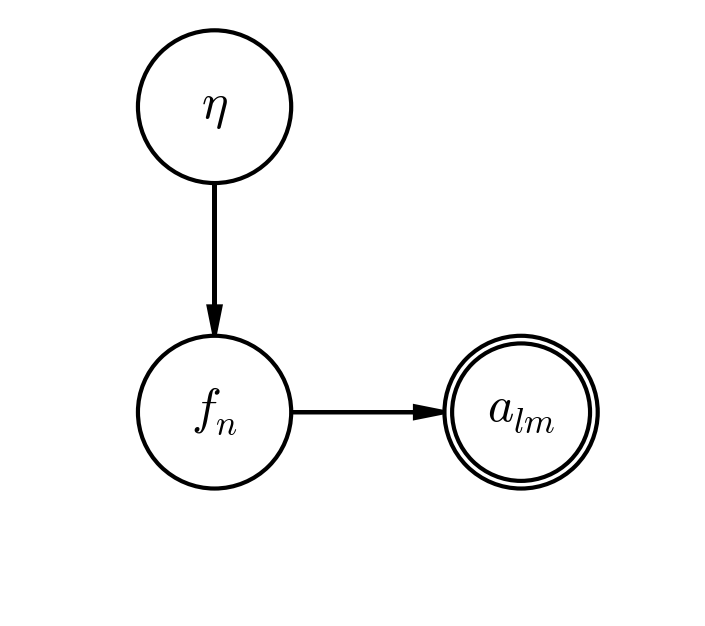
\includegraphics[width=0.50\textwidth]{figures/inflation.png}\\
\caption{\label{inflationPGM} Probabilistic graphical model for the joint distribution $\mathcal{P}(a_{lm},\,f_n,\,\vec{\eta} )$.
}

\end{center}
\end{figure*}

The quantity we are after is $\mathcal{P}(\vec{\eta}| a_{lm})$, which is marginalized over the potential map (the $f_n$s). We therefore proceed as follows:
%  \be
% 	\mathcal{P}(\vec{\eta}| a_{lm} )=\frac{\mathcal{P}(\vec{\eta})}{\mathcal{P}( f_n, \, a_{lm})}\int \mathrm{d}f_n\mathcal{P}( a_{lm}| f_n) \mathcal{P}( f_n|\vec{\eta})
% \ee
 \bea
 	\mathcal{P}(\vec{\eta}| a_{lm} )&=& \int \mathrm{d}f_n\, \mathcal{P}(\vec{\eta}| f_n, a_{lm}) \mathcal{P}(f_n | a_{lm}) \, ,
	\\
	&=&\frac{\mathcal{P}(\vec{\eta})}{\mathcal{P}(a_{lm})}\int \mathrm{d}f_n\mathcal{P}( a_{lm}| f_n) \, .\mathcal{P}( f_n|\vec{\eta})
 \eea

We have:
\be
\label{eq:aPDF}
	\mathcal{P}( a_{lm}| f_n) =\frac{1}{\sqrt{(2\pi)^{p}\mathrm{Det}(C_a)}} \exp\left[ -\frac{1}{2}\left(a_{lm}-\mathbf{R} f_n\right)^{\mathrm{T}}C^{-1}_a\left(a_{lm}-\mathbf{R} f_n\right)\right]\, ,
\ee
where $p=l_{max}^2+2l_{max}+1$ is the total number of independent measurements in $a_{lm}$ up to the harmonic $l_{max}$. Assuming the CMB fluctuations are Gaussian, the $f_n$s are described by a Gaussian distribution with variance given by the inflationary power spectrum:
\be
\label{eq:fnPDF}
	\mathcal{P}( f_n|\vec{\eta})= \sqrt{\frac{\mathrm{Det}(C_f^{-1})}{(2\pi)^{n_{tot}}}}\exp\left[ f_n^{\mathrm{T}}C_f^{-1}f_n \right]\,,
\ee
with $C_f^{-1}$ a diagonal matrix given by:
\be
\label{eq:fncovariancematrix}
	C_f^{-1}  =\left(  \begin{array}{ccccccc} 1/\sigma_{n_1}^1&0&0&... &0 &...&0\\ 0& 1/\sigma_{n_2}^2 &0& &... \\ ... & & & &\\ 0&...&  & &1/\sigma_{n_i}^2\\
	...&&&&&...&\\
	0&&&&&&1/\sigma_{n_{tot}}^2
	\end{array} \right)\, ,
\ee
where the $\sigma_{n_i}$ only depend on the norm of the $\vec{n}_i$ vector to which they correspond (or equivalently on the norm or the corresponding Fourier mode $|\vec{k}|$). More specifically, they are given in terms of the power spectrum by:
\bea
	\sigma_k^2&=&\mathcal{P}_\zeta(k)\nonumber\\
	&=&\frac{1}{4k^{3}}\frac{V(\varphi_*)\left[1+d_1\frac{\Delta\varphi}{\Mp}+\frac{1}{2}d_2\frac{\Delta\varphi^2}{\Mp^2}+\frac{1}{3!}d_3\frac{\Delta\varphi^3}{\Mp^3} +\frac{1}{4!}d_4\frac{\Delta\varphi^4}{\Mp^4}\right]}{\Mp^2\left( \epsilon_*+\Gamma_1\frac{\Delta\varphi}{\Mp}+\frac{\Gamma_2}{2}\frac{\Delta\varphi^2}{\Mp^2}+\frac{\Gamma_3}{3!}\frac{\Delta\varphi^3}{\Mp^3}+\frac{\Gamma_4}{4!}\frac{\Delta\varphi^4}{\Mp^4})\right)\left(3-\epsilon_*+\Gamma_1\frac{\Delta\varphi}{\Mp}+\frac{\Gamma_2}{2}\frac{\Delta\varphi^2}{\Mp^2}+\frac{\Gamma_3}{3!}\frac{\Delta\varphi^3}{\Mp^3}+\frac{\Gamma_4}{4!}\frac{\Delta\varphi^4}{\Mp^4}\right)}\, .
\eea
Here, the mapping between $k$ and $\Delta \varphi$ has to be done using equation (\ref{eq:kDeltavarphimapping}). We therefore obtain that the $f_n$ covariance matrix only depends on the $\vec{\eta}$ vector.

To completely define the problem, we are left with the task of specifying a prior on $\vec{\eta}$.  First, the energy scale of inflation must lie between the BBN scale and (hopefully) the string scale. Actually, given the observed amplitude of the power spectrum, we can safely lower the upper bound by two orders of magnitude. Therefore, we know $\rho=3H^2\Mp^2$ should lie within $\left[ (10^{17}\mathrm{GeV})^4, \, (10 \, \mathrm{TeV})^4 \right]$. This can be translated into an allowed range of $H$ values, $[2.4\times 10^{-14}\mathrm{eV} ,\,2.4\times10^{15}\mathrm{GeV}]$. Note that these values are taken for the parameters at the time when the scale $k=0.05$Mpc$^{-1}$ exited the Hubble horizon during inflation.

Because of this huge range of allowed $H$ values, and because we expect $H_*$ and $\epsilon_*$ to be degenerate since only their ratio appears in the expression for the power spectrum, it is convenient to change variables in our inflationary parameter vector as follows:
\be
	\vec{\eta}=\left(\frac{H^2_*}{\epsilon_*},\, \epsilon_*, \,\eta_*, \, (\eta_2)_*, \,(\eta_3)_*\right)\, .
\ee
We make this choice of parametrization for the first element of $\vec{\eta}$ because we expect the amplitude of the power spectrum to be well-constrained by the data $a_{lm}$, whereas $H_*$ and $V(\varphi_*)$, while degenerate with $\epsilon_*$, are easily obtained from the $\Delta^2_\zeta(k_*)$ amplitude once a value of $\epsilon_*$ is picked:
\bea
	\frac{H^2_*}{\epsilon_*}=8\pi^2\Mp^2\Delta^2_\zeta(k_*)\quad&\Rightarrow&\quad H_*=\sqrt{\Delta^2_\zeta(k_*)\, 8\pi^2\epsilon_*(2.435\times10^{18}\mathrm{GeV})^2}\, ,\\
	&\&&\quad V(\varphi_*)=H_*^2 \,(2.435\times10^{18}\mathrm{GeV})^2 \, (3-\epsilon_*)
\eea
where we used $\Mp=2.435\times10^{18}\mathrm{GeV}$.

We finally arrive at the following set of constraints on the parameters of the new $\vec{\eta}$ vector:
\be
\label{eq:priors}
	\left\{\begin{array}{ccl} %H^2_*/\epsilon_*&\varepsilon & \left[ 8\pi^2\Mp^2 10^{-9},\,  8\pi^2\Mp^2 10^{-8}\right] \\
	\epsilon_* &\varepsilon& \left[10^{-76},\, 1 \right[\\
	\eta_*  &\varepsilon& \left]-1,\, 1 \right[\\
	(\eta_2)_*  &\varepsilon& \left[-1,\, 1 \right]\\
	|(\eta_3)_*|  &<& |(\eta_2)_*|
	\end{array} \right.
\ee
and
\be
	\mathcal{P}(x\equiv H^2_*/\epsilon_*)=\frac{1}{(\sigma=0.22)\sqrt{2\pi}}\exp\left[-\frac{1}{2}\frac{(x-(\mu=2.43))^2}{(\sigma=0.22)^2}�\right]\, .
\ee
These are very conservative bounds. The bound on $ H^2_*/\epsilon_*$ is taken to be a wide Gaussian centered on the WMAP7 value of $\Delta^2_\zeta=(2.43\pm0.11)\times10^{-9}$ at the pivot scale $k_0=0.02$Mpc$^{-1}$. The lower bound on $\epsilon_*$ is calculated from the lower bound on the energy scale of inflation. The rest of the bounds are drawn only from the requirement that the slow-roll approximation holds. This should be the case since the low $k$ values that we are interested in here correspond to the first few of the 60 $e$-folds of inflation that should have occurred to solve e.g. the flatness and homogeneity problems. For example, $\epsilon<1$ is equivalent to the statement the Universe is inflating, and $|\eta|\leq1$ translate to the requirement that inflation can last for long enough. $\eta_2$ and $\eta_3$ being higher-order parameters, it is then expected that they should be somewhat smaller. It would be possible put a somewhat stronger prior on $\epsilon_*$ using the bound on $r$ from the latest Planck results, however this bound is for a different scale from the one we are looking at here (i.e. the first acoustic peak in the power spectrum), and it varies a lot depending on the assumptions made on other parameters (e.g. the running of the power spectrum).

%To get a specific range of allowed $V(\varphi_*)$, in (\ref{eq:priors}) we first used the normalization of the power spectrum at the scale $k_*$ (which I believe was called $\alpha$) and the allowed range of $\epsilon_*$ to obtain a ranged of allowed $H_*$
%\be
%	\alpha=\frac{H^2_*}{8\pi^2\epsilon_*\Mp^2}\quad\Rightarrow\quad H_*=\sqrt{2.4\times10^{-9}\, 8\pi^2\epsilon_*(2.435\times10^{18}\mathrm{GeV})^2}\, ,
%\ee
%where we used $\alpha=2.4\times10^{-9}$ and $\Mp=2.435\times10^{18}\mathrm{GeV}$. From there, the range of values of $V(\varphi_*)$ can be found as follows
%\be
%	H_*^2\Mp^2 (3-\epsilon_*)=V(\varphi_*)\quad\Rightarrow\quad V(\varphi_*)\quad\varepsilon\quad[10^{57}\mathrm{GeV}^4,\, 1.5\times10^{68}\mathrm{GeV}^4]
%\ee
\bigskip

Performing the integral over $\mathrm{d}f_n$, we obtain (see handwritten notes for details):
\bea
	\mathcal{P}(\vec{\eta}| a_{lm} )&=&\sqrt{\frac{\mathrm{Det}(C_f^{-1})}{(2\pi)^{n_{tot}}}}\frac{1}{\sqrt{(2\pi)^{p}\mathrm{Det}(C_a)}} \frac{(2\pi)^{(n_{tot}/2)}}{(\mathrm{Det}\,\mathbf{A})^{1/2}}\exp\left\{\frac{1}{2}\mathbf{B}^{\mathrm{T}}\mathbf{A}^{-1}\mathbf{B}-\frac{1}{2}a^{\mathrm{T}}_{lm}C_a^{-1}a_{lm} \right\}\frac{\mathcal{P}(\vec{\eta})}{\mathcal{P}(a_{lm})}\, , \\
	&=&\frac{1}{(2\pi)^{p/2}} \frac{1}{\left[\mathrm{Det}(C_f)\mathrm{Det}(C_a)\mathrm{Det}\,\mathbf{A}\right]^{1/2}}\exp\left\{\frac{1}{2}\mathbf{B}^{\mathrm{T}}\mathbf{A}^{-1}\mathbf{B}-\frac{1}{2}a^{\mathrm{T}}_{lm}C_a^{-1}a_{lm} \right\}\frac{\mathcal{P}(\vec{\eta})}{\mathcal{P}(a_{lm})}\, ,
\eea
where the $\mathbf{A}$ and $\mathbf{B}$ matrices are given by:
\bea
	\mathbf{A}~~&=&\mathbf{R}^{\mathrm{T}}C^{-1}_a \mathbf{R}+C_f^{-1}\\
	 \mathbf{B}^{\mathrm{T}}&=&a_{lm}^{\mathrm{T}}C_a^{-1}\mathbf{R}
\eea

%%%%%%%%%%%%%%%%%%%%%%%%%%%%%%%%%%%%%%%%%%%%%%%%%%%%%%%%%%%%%%%%%%%%%%

\section{Potential map inference}

We are also interested in inferring the potential maps from the $f_n$, given the data $a_{lm}$ and an assumed prior on the $f_n$s given by (\ref{eq:fnPDF}) with the covariance matrix (\ref{eq:fncovariancematrix}). We write
\be
	\mathcal{P}(f_n | a_{lm}, \vec{\eta}, C_f^{-1})=\frac{\mathcal{P}(a_{lm}|f_n) \mathcal{P}(f_n|  \vec{\eta}, C_f^{-1})}{\mathcal{P}(a_{lm}| \vec{\eta}, C_f^{-1})}\, .
\ee

\begin{figure*}[H]
\begin{center}
\centering
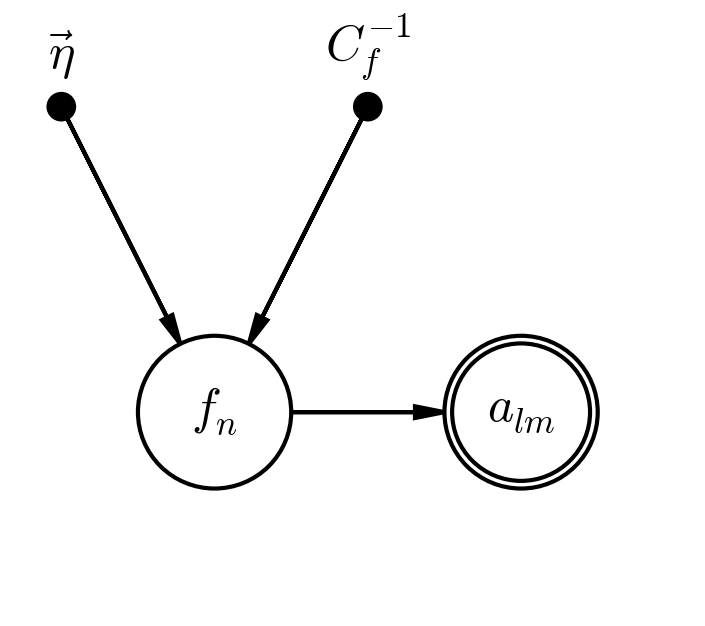
\includegraphics[width=0.50\textwidth]{figures/simple-map.png}\\
\caption{\label{simplepng} Probabilistic graphical model for the joint distribution $\mathcal{P}(a_{lm},\,f_n |\vec{\eta}, C_f^{-1} )$.
}

\end{center}
\end{figure*}

The PGM for this inference is given in figure \ref{simplepng}. The numerator is given by (\ref{eq:aPDF}) and (\ref{eq:fnPDF}). Completing the square, we can rewrite this expression as:
\bea
	&\mathcal{P}&(f_n | a_{lm}, \vec{\eta}, C_f^{-1})=\\
	&&\exp\left[-\frac{1}{2} \left( f_n^T-a^T_{lm}C_a^{-1}\mathbf{R}\mathbf{A}^{-1} \right) \mathbf{A}\left(f_n-\mathbf{A}^{-1}\mathbf{R}^TC_a^{-1} a_{lm} \right) \right]\exp\left[\frac{1}{2} a_{lm}^T\left(C_a^{-1}\mathrm{R} \mathrm{A}^{-1} \mathrm{R}^TC_a^{-1} -C_a^{-1} \right) a_{lm} \right]\, .
\eea
From this, we can read the most likely values of the $f_n$s,
\be
	\langle f_n \rangle=\mathbf{A}^{-1}\mathbf{R}^TC_a^{-1} a_{lm}\, .
\ee


%%%%%%%%%%%%%%%%%%%%%%%%%%%%%%%%%%%%%%%%%%%%%%%%%%%%%%%%%%%%%%%%%%%%%%

\newpage
\section{Appendix A: Calculating the minimum value of $\epsilon_*$ from stochastic noise}

Bottom line: there is no model-independent minimum value of $\epsilon_*$ coming form the stochastic contribution of $\varphi$ to the background evolution.

To see this, we decompose $\epsilon_*$ into a classical piece, $\epsilon_{C*}$, and a stochastic piece, $\epsilon_{\xi*}$,
\bea
\label{eq:epsilonsplitdotvarphi}
	\epsilon_*=\epsilon_{C*}+\epsilon_{\xi*}&= &\frac{\dot\varphi_*^2}{2\Mp^2H_*^2}+\frac{\dot\varphi_*}{2\pi}\tilde{\xi}\, ,
\eea
where $\tilde\xi$ is white noise with mean zero and variance 1. The first term on the r.h.s. of the above equation still has a stochastic piece. In order to cleanly separate $\epsilon_{C*}$ and $\epsilon_{\xi*}$, we make use of the stochastic equation of motion for $\varphi$
\be
	\dot\varphi=-\frac{V_{,\varphi}}{3H}+\frac{H^2}{2\pi}\tilde\xi\, .
\ee
We then obtain
\be
\label{eq:splitepsilonstar}
	\epsilon_*=-\frac{V_{,\varphi_*}^2}{2\Mp^29H_*^4}-\frac{V_{,\varphi_*}}{12\pi H_*\Mp^2}\tilde{\xi}\, .
\ee
Now, $V_{,\varphi}$ possibly still has some stochastic piece (this is a model-dependent statement: for some models it is purely classical), but in cases where we remain away from eternal inflation, that piece should remain small. Requiring that the $\epsilon_*$ allowed by our prior distribution aren't the ones describing eternal inflation is sensible (since we know that in our Hubble patch, inflation ended!)

\subsubsection{$\lambda\varphi^n$ - class of models}
To see how this works out in the case of a specific model of inflation, take the class of chaotic models with $V=\lambda\varphi^n$. The two terms of (\ref{eq:splitepsilonstar}) can be re-expressed as follows:
\\
First term:
\be
	\frac{V_{,\varphi_*}^2}{2\Mp^29H_*^4}=\frac{\left(\lambda\varphi_*^{(n-1)}\right)^2}{9H_*^22\Mp^2}\left(\frac{\lambda \varphi_*^n}{3\Mp^2}\right)^{-1}=\frac{n\lambda}{6 H_*^2}\varphi^{(n-2)}_*=\frac{n\Mp^2}{2\varphi_*^2}\, .
\ee
Second term:
\be
	\frac{V_{,\varphi_*}}{12\pi H_*\Mp^2}\tilde{\xi}=\frac{n\lambda\varphi_*^{(n-1)}}{12\pi H_*\Mp^2}\tilde\xi= \frac{nH_*}{2\pi\varphi_*}\tilde\xi=\frac{n}{2\pi}\sqrt{\frac{\lambda}{3}}\frac{\varphi_*^{(\frac{n}{2}-1)}}{\Mp}\, .
\ee

Looking at the first term first, we can expand $\varphi_*$ itself into a classical piece and a stochastic piece, $\varphi_*=\varphi_{cl\,*}+W_*$, and, assuming that we are outside of the regime of eternal inflation, we can safely assume $\varphi_{cl\,*}\gg W_*$. Therefore, the first term of (\ref{eq:splitepsilonstar}) becomes:
\be
	\frac{V_{,\varphi_*}^2}{2\Mp^29H_*^4}\approx \frac{n}{2}\frac{\Mp^2}{\varphi_{cl\,*}^2}\left( 1-2 \frac{W_*}{\varphi_{cl\, *}}\right)\, ,
\ee
and the stochastic contribution of this term to $\epsilon_{\xi*}$ is therefore
\be
	\epsilon_{\xi*}  ~ \supset~ n\frac{\Mp^2}{\varphi_{cl\,*}^2}\left(  \frac{W_*}{\varphi_{cl\, *}}\right)\, .
\ee
The remain part, $ \frac{n}{2}\frac{\Mp^2}{\varphi_{cl\,*}^2}$, is then the classical $\epsilon_{C*}$. We then see that this stochastic contribution to the first slow-roll parameter is always smaller than its classical countrepiece, and therefore from theoretical grounds, it can be tuned arbitrarily close to zero.

Turning to the second term in (\ref{eq:splitepsilonstar}), and expanding $\varphi_*$ in a similar way as above, we obtain:
\bea
	\frac{V_{,\varphi_*}}{12\pi H_*\Mp^2}\tilde{\xi}&\approx&  \frac{n}{2\pi}\sqrt{\frac{\lambda}{3}}\frac{\varphi_{cl\,*}^{(\frac{n}{2}-1)}}{\Mp}\left(1+\frac{n-2}{2}\frac{W_*}{\varphi_{cl\,*}} \right)\tilde\xi \, ;\\
	&\approx&\frac{n}{2\pi}\sqrt{\frac{\lambda}{3}}\frac{\varphi_{cl\,*}^{(\frac{n}{2}-1)}}{\Mp}\tilde\xi \, .
\eea
This is a pure contribution to $\epsilon_{\xi\, *}$. Even if the ratio $\varphi/\Mp$ could potentially be large provided the slow-roll condition is satisfied, the $\sqrt{\lambda}$ pre-factor can be tuned arbitrary close to zero, and therefore there is no minimum value of $\epsilon_*$ from a theoretical standpoint.

\subsubsection{Model-independent case}
To derive a model-independent statement, we need to find a model-independent expression for $\dot\varphi_*$.
From (\ref{eq:epsilonsplitdotvarphi}), we get
\be
	\dot\varphi_*=\frac{\tilde\xi H_*^2}{4\pi}+H_*\Mp\sqrt{2\epsilon_*+\frac{H^2_*}{(4\pi)^2}\frac{\tilde\xi^2}{\Mp^2}}
\ee
Plugging this into Friedmann equation, we can get an expression for $V(\varphi_*)$:
\be
	3H^2_*\Mp^2=\frac{1}{2}\left[\frac{H_*^4\tilde\xi_*^2}{(4\pi)^2} +\frac{H^3_*\Mp}{2\pi}\tilde\xi\sqrt{2\epsilon_* +\frac{H^2_*\tilde\xi^2}{(4\pi)^2\Mp^2}} +H_*^2\Mp^2\left(2\epsilon_*+\frac{H^2_*}{(4\pi)^2}\frac{\tilde\xi^2}{\Mp^2}\right)\right]+V(\varphi_*)\, .
\ee
From here, it is easy (but tedious) to derive an expression for $V_{,\varphi_*}$
\bea
	V_{,\varphi_*}&=& -\Mp H^2_*\sqrt{\frac{\epsilon_*}{2}}(6-2\epsilon_*+\eta_*)+H^2_*\left[ \frac{H_*}{4\pi}\tilde\xi +\Mp\sqrt{2\epsilon_*+\frac{H^2_*}{(4\pi)^2}\frac{\tilde\xi^2}{\Mp^2}}\right]^{-1}\nonumber\\
	&&\qquad\times\left[ \frac{H^2\epsilon_*}{4\pi^2}\tilde\xi - \frac{\epsilon_*H_*\Mp}{2\pi}\sqrt{2\epsilon_*+\frac{H^2_*}{(4\pi)^2}\frac{\tilde\xi^2}{\Mp^2}}-\frac{H_*\Mp}{8\pi}\frac{(2\epsilon_*\eta_*-\tilde\xi^2\frac{H^2_*}{\Mp^2}\frac{\epsilon_*}{2\pi})}{\sqrt{2\epsilon_*+\frac{H^2_*}{(4\pi)^2}\frac{\tilde\xi^2}{\Mp^2}}} \right]\, .
\eea
From here, we see that all terms in $V_{,\varphi_*}$ are proportional to at least one power of the slow-roll parameters, even the stochastic ones. Therefore, by tuning the classical value of $\epsilon_*$ arbitrarily close to zero, it's possible to make the stochastic contribution also arbitrarily close to zero, hence there is no minimum value of epsilon coming form stochastic effects.

%%%%%%%%%%%%%%%%%%%%%%%%%%%%%%%%%%%%%%%%%%%%%%%%%%%%%%%%%%%%%%%%%%%%%%

\end{document}

%%%%%%%%%%%%%%%%%%%%%%%%%%%%%%%%%%%%%%%%%%%%%%%%%%%%%%%%%%%%%%%%%%%%%%
